\Lecture{Sunil K S}{Jan 24, 2012}{10}{Polynomial Identity Testing}

Towards the end of last lecture, we introduced the following problem :
{\em Given a polynomial $p$, test if it is identically zero}. That is,
do all the terms cancel out and become the zero polynomial. Described
as a language :
$$\textrm{\sc PIT}=\{ p ~|~p \equiv 0\}$$
We also saw some easy cases of the problem:
\begin{enumerate}
\item When it is given as a sum of monomials: Given $p$, run over the
  input to figure out the coefficient of each monomial, and if all of
  them turn out to be zero, then report that $p$ is in {\sc PIT}. This
  algorithm runs in $O(n^2)$ time.
\item When it is given as a Black Box: In uni-variate case, check
  $p(x)$ for $d+1$ different points where $d$ is the degree bound. If
  the polynomial is not equivalent to zero, then at-least one of the
  steps gives a non-zero value. Indeed, if the polynomial is zero,
  then all the $(d+1)$ evaluations will result in a zero value. Thus
  the algorithm is correct and runs in time $O(d)$ where $d$ is the
  degree of the polynomial.
\end{enumerate}

As we observed, this strategy could not be generalized in
multi-variate case. We took an example as $p(x_1,x_2) = x_1x_2$. For
the assignment $x_1=0$, whatever $x_2$ chose, the value will always be
0. However, if $p \equiv 0$, no matter what we choose as the
substitution for $x_1$, and $x_2$, the polynomial will be identically
zero.

The strategy that we will follow is as follows: If the total degree of
the polynomial is $\leq d$, and if $S \subseteq \F$, such that
$|S|\geq 2d$, instead of picking elements arbitrarily, we pick
elements uniformly at random from $S$. Indeed, there may be many
choices for the values which may lead to zero. But how many?
%Here by increasing the size of $S$, we can improve the probability.
% IMPRECISE statement.

\begin{lemma}[Schwartz-Zippel Lemma]
Let $p(x_1, x_2, \cdots , x_n)$ be a non-zero polynomial over a field
$\mathbb{F}$. Let $S\subseteq \mathbb{F}$
$$Pr[p(\bar{a}=0]\leq \frac{d}{|S|}$$
\end{lemma}
%It also shows that the number of solutions for $P(\bar{a})$ if $\leq d|S|^{(n-1)}$.
\begin{proof}
(By induction on $n$) For $n=1$: For a univariate polynomial $p$ of
  degree $d$, there are $\leq d$ roots. Now in the worst case the set
  $S$ that we picked has all $d$ roots. Thus for a random choice of
  substitution for the variable from $S$, the probability that it is a zero of
  the polynomial $p$ is at most $\frac{d}{|S|}$.

For $n>1$, write the polynomial $p$ as a univariate polynomial in $x_1$ with coefficients as polynomials in the variables $p(x_2, \ldots, x_n)$.
$$ \displaystyle \sum_{j=0}^{d}x_1^jp_j(x_2, x_3, \ldots, x_n)$$

For example: $x_1x_2^2+x_1^2x_2x_3+x_3^2=(x_2x_3)x_1^2+(x_2^2)x_1+x_1^0(x_3^2)$.

To analyse the probability that we will choose a zero of the
polynomial (even though the polynomial is not identically zero). For a
choice of the variables as $(a_1, a_2, \cdots, a_n)\in S^n$, we ask
the question : how can $p(a_1, a_2, \cdots, a_n)$ be zero? It could be
because of two reasons:

\begin{enumerate}
\item $\forall j~:~1 \le j \le n , ~~ p_j(a_2, a_3, \ldots , a_n)=0$.
% In this case whatever $(a_2, a_3, \cdots , a_n)=0$, polynomial will be zero.
\item %$(a_2, a_3, \cdots , a_n)=0$.
Some coefficients $p_j(a_2, a_3, \ldots , a_n)=0$ are non-zero, but
the resulting univariate polynomial in $x_1$ evaluates to zero upon
substituting $x_1 = a_1$.
\end{enumerate}

Now we are ready to calculate $Pr [ p(a_1, a_2, \ldots, a_n) = 0 ]$.
%\begin{eqnarray*}
For a random choice of $(a_1, \ldots, a_n)$.
Let $A$ denote the event that the polynomial $p(a_1, \ldots, a_n) = 0$.
Let $B$ denote the event that $\forall j~:~1 \le j \le n ,~~p_j(a_2, a_3, \cdots , a_n)=0$.
Now we simply write : $Pr[A] = Pr[A \land B]+Pr[A\land \bar{B}]$.

We calculate both the terms separately: $Pr[A \land B] = Pr[B].Pr[A|B]
= Pr[B]$ where the last equality is because $B \implies A$.  Let
$\ell$ be the highest power of $x_1$ in $p(x)$. That is $p_\ell \ne
0$. Since the event $B$ insists that for all $j$, $p_j(a_2, a_3,
\ldots , a_n)=0$, we have that $Pr[B] \leq Pr[p_\ell(a_1, a_2, \ldots,
  a_n) \ne 0]$.  By induction hypothesis, since this polynomial has
only $n-1$ variables and has degree at most $\frac{d -
  \ell}{S}$. Thus, $Pr[B] \le \frac{d - \ell}{S}$.

To calculate the other term,
\begin{eqnarray*}
Pr[A \cap \bar{B}] & = & Pr[\bar{B}].Pr[A|\bar{B}] \le Pr[A|\bar{B}] \le \frac{\ell}{|S|}
\end{eqnarray*}
where the last inequality holds because the degree of the non-zero
univariate polynomial after substituting for $a_2, \ldots, a_n$ is at
most $\ell$ and hence the base case applies.
\end{proof}

This suggests the following efficient algorithm for solving PIT. Given $d$ and a
blackbox evaluating the polynomial $p$ of degree at most $d$.

\begin{figure}[ht]
{\tt \obeyspaces \obeylines
1. Choose $S \subseteq \mathbb{F}$ of size $\ge 4d$.
1. Choose $(a_1, a_2, \ldots, a_n) \in_R S^n$.
2. Evaluate $p(a_1, a_2, \ldots a_n)$ by querying the blackbox.
3. If it evaluates to 0 accept else reject.
}
\caption{A randomized algorithm for multivariate polynomial identity testing}
\end{figure}

The algorithm is clearly running in polynomial time. The following
Lemma states the error probability and follows from the
Schwartz-Zippel Lemma that we saw before.
\begin{lemma}
There is a randomized polynomial time algorithm $A$, which, given a black
box access to a polynomial $p$ of degree $d$ ($d$ is also given in unary), answers whether the polynomial is identically zero or not,
with probability at least $\frac{3}{4}$.
%\[ p \not\equiv 0 \implies \textrm{ Pr[$A$ accepts] $\ge \frac{3}{4}$} \]
%\[ p \equiv 0 \implies \textrm{ Pr[$A$ accepts] $= 0$.} \]
\end{lemma}

Notice that in fact the lemma is weak in the sense that it ignores the
fact that when the polynomial is identically zero then the success
probability of the algorithm is actually 1 !.

Now we connect to where we left out from Branching machines, by
observing that this randomized algorithm is indeed a branching machine.
Let $\chi_L(x)$ denote the characterestic function of the
language. That $\chi_L(x) = 1$ if $x \in L$ and $0$ otherwise.  Let us
call a computation path to be {\em erroneous} if the decision ($1$ for
accept and $0$ for reject) reported in that path is not
$\chi_L(x)$.  Let $\#err_M(x)$ denote the number of erroneous paths.
Thus the braching machine has some guarantees about $\#err_M(x)$.
%with some guarantees on the number of erroneous paths.

\begin{corollary}
Let $L$ be the language $PIT$, then there exists a branching machine
$M$, running in $p(n)$ time (hence using at most $p(n)$ branching
bits).
\[ \#err_M(x) \le \frac{1}{4}2^{p(n)} \]
%\begin{eqnarray*}
%x\in L&\Rightarrow&     \#acc_M(x)\geq \frac{3}{4}2^{p(n)}. \mbox{ In case of PIT, it is } =2^{p(n)}.\\
%x\notin L&\Rightarrow&  \#acc_M(x)\leq \frac{1}{4}2^{p(n)}.% \mbox{ } \rightarrow P\neq 0.
%\end{eqnarray*}
\end{corollary}

Is there anything special about $\frac{1}{4}$? As we can go back an
observe, this number can be reduced to say $\frac{1}{5}$ by easily
choosing the size of the set $S$ to be larger than $5d$ where $d$ is
the degree of the polynomial. We get better success probability then,
but what do we lose? We lose on the running time, since we have to
spend more time and random bits now in order to choose the elements
from $S^n$ as $|S|$ has gone up.

But more seriously, this seems to be an adhoc method which applies
only to this problem. In general, if we have a randomized algorithm
that achieves a success probability of $\frac{3}{4}$, can we boost it
to another constant?

Based on the discussion so far, we can make the following definition
of a set of languages. For a fixed $\epsilon$, define the class $\BPP_\epsilon$ as follows.
%\textbf{Bounded error Probabilistic Polynomial time (BPP)}:\\ 
$L \in BPP_{\epsilon}$, for some $0 \epsilon < \frac{1}{2}$, if there is a branching machine $M$
running in time $p(n)$, such that $\#err_M(x) \le \epsilon2^{p(n)}$.

Notice that all these sets of classes are contained in $\PSPACE$. Let $L \in
BPP_{\epsilon}$ via a machien $M$.  By just brute force run over all
the choice bits of the machine $M$ (reusing space across different
paths) we can exactly calculate how many paths are accepting. This
information will be sufficient to decide whether $x \in L$ or not..

All of them contain $\P$ since there is a trivial choice machine which
achieves any success probability (of 1 !).

How do they compare, for different $\epsilon$ and $\epsilon'$? Could
they be incomparable with each other (and hence form an antichain in
the poset of languages)? In the next lecture we will show a lemma
which will imply that for any constants $0 < \epsilon \ne \epsilon' <
\frac{1}{2}$, $\BPP_\epsilon = \BPP_{\epsilon'}$.  This eliminates the
possibility of an antichain in the poset and makes the definition of
the following complexity class.

\begin{definition}[BPP]
A language $L$ is said to be in $\BPP$ if there is an $\epsilon$ such
that $0 < \epsilon \le \frac{1}{2}$, and a branching machine $M$
running in time $p(n)$ such that: $\#err_M(x) \le \epsilon2^{p(n)}$
\end{definition}

We begin the thoughts on proving $\BPP_\epsilon = \BPP_{\epsilon'}$
for $0 < \epsilon \ne \epsilon' < \frac{1}{2}$. Without loss of
generality, assume that $\epsilon < \epsilon'$.  Note that
$\BPP_\epsilon \subseteq \BPP_{\epsilon'}$. To show the other
direction we need to improve the success probability of the
algorithm. Viewing the success of the algorithm as a favourable
probability event, a natural strategy is to repeat the process
independently again, so that the probability of error goes down
multiplicatively. Thus it improves the success probability.

%\begin{figure}[htb]
%\begin{center}
%\scalebox{0.8}{ 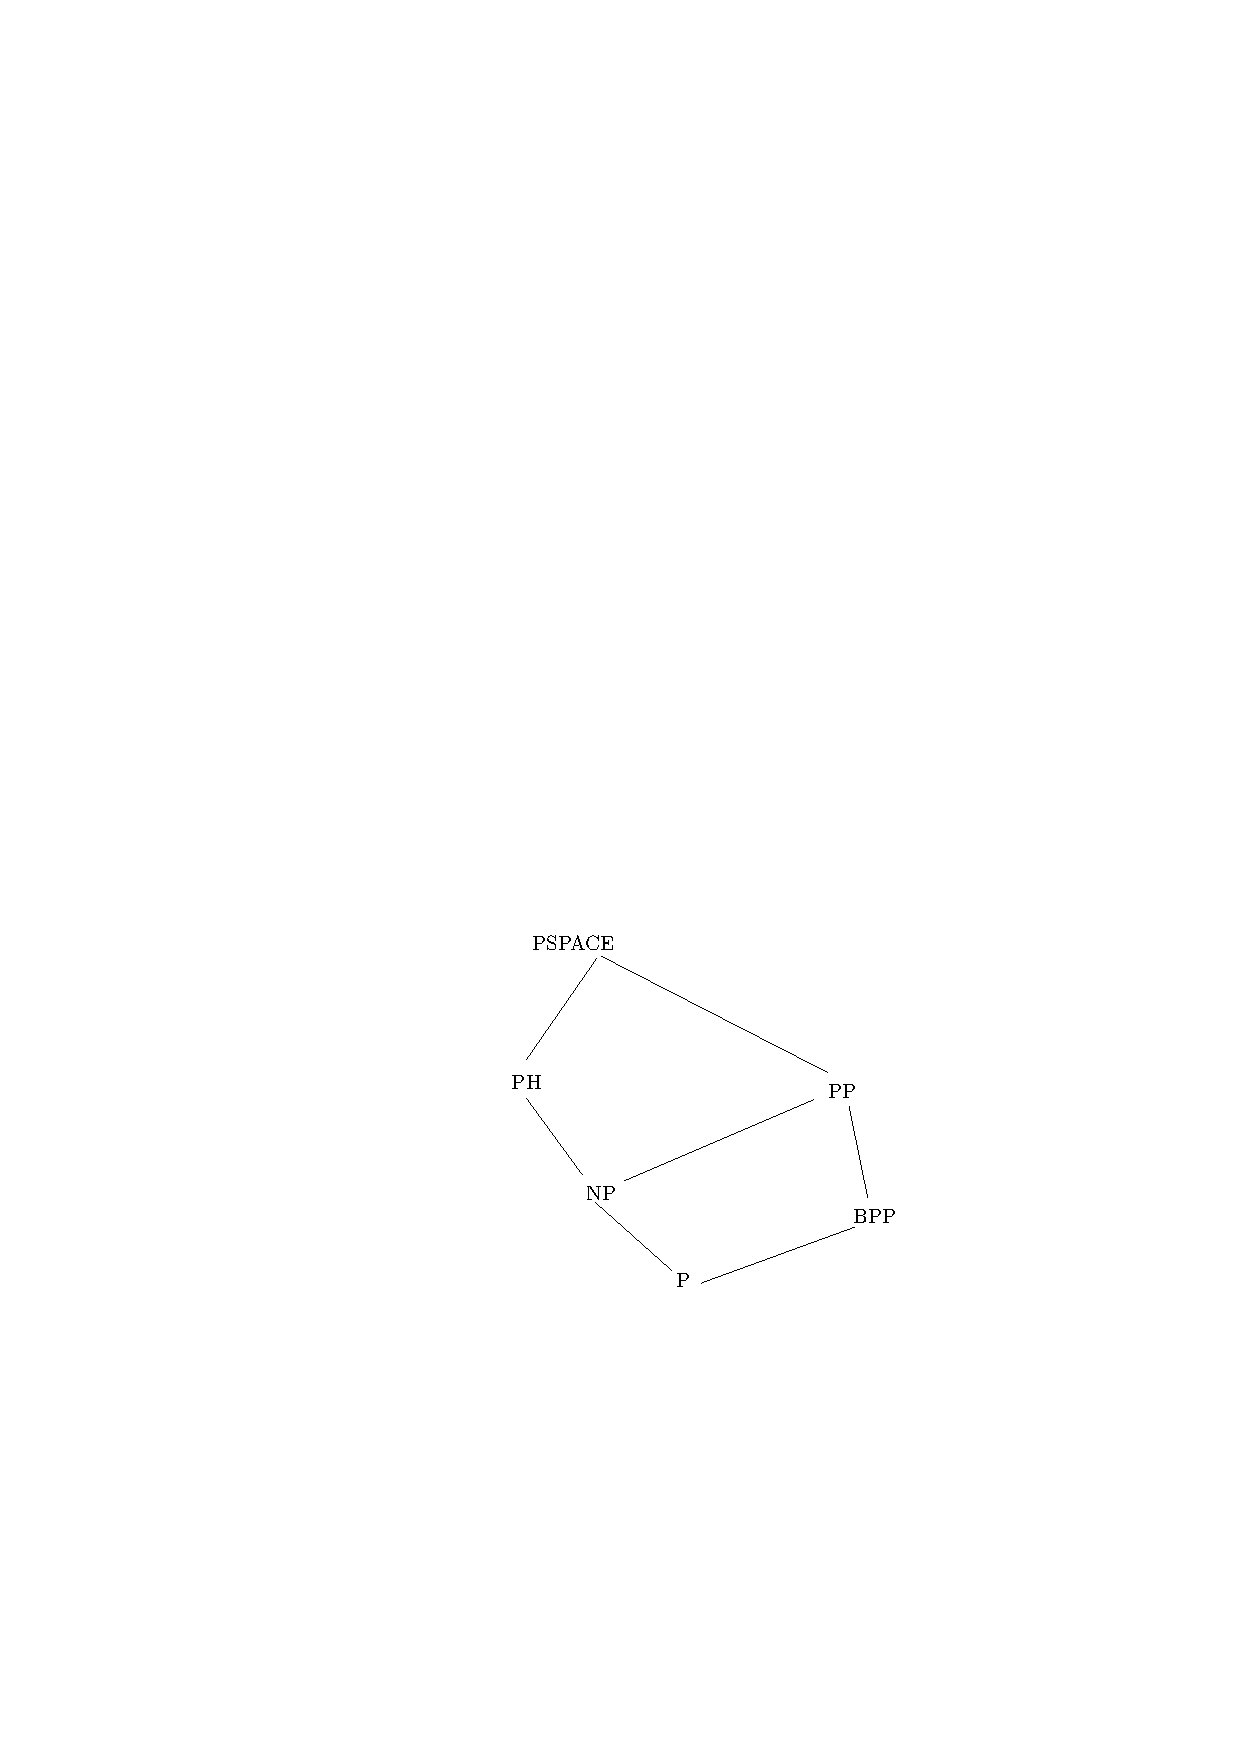
\includegraphics{1.pdf} }
%\end{center}
%\caption{Different Complexity Classes.}
%\label{complexity}
%\end{figure}

